\section{Frequentist vs Bayesian Thinking}

Let's start with the \textit{Frequentist definition of probability}. In this approach, probability is based on the observation of a large number of trials. Imagine you're flipping a coin. The probability of getting heads, which we will call \textit{event} \(E\), is denoted by \(P(E)\). Now, if you flip the coin \(n\) times and observe that you get heads \(n_E\) times, the frequentist probability is given by the ratio of the number of heads to the total number of flips. Mathematically, this is expressed as:

\[
P(E) = \lim_{n \to \infty} \frac{n_E}{n}.
\]

What this formula means is that as you keep flipping the coin over and over, the ratio of heads to total flips should converge to a particular value, which we call the probability of heads. The more trials you conduct, the closer you get to this true probability.\\

On the other hand, the \textit{Bayesian definition of probability} is quite different. In the Bayesian framework, probability is not based solely on repeated trials but rather reflects our \textit{beliefs} or \textit{knowledge} about an event. So, for a Bayesian, \(P(E)\) can be any probability distribution as long as it's consistent with prior beliefs. For instance, if you believe the probability of a coin landing heads is 0.7, you can start with that assumption, and update your belief as you gather more evidence.\\

Now, let's move to \textit{inference}. The frequentist and Bayesian approaches lead to different methods of making inferences.\\

In the frequentist world, we talk about \textit{confidence intervals}. A confidence interval is a range of values where we expect the true population parameter to lie based on repeated random samples. For example, if you generate 100 random samples, and 95 of those samples contain the true value, then you have a 95\% confidence level. Importantly, the confidence level \textit{does not} mean that there's a 95\% chance the true value is in any given interval. Instead, 95\% of similarly constructed intervals will contain the true value.\\

Let’s consider a real-world example based on a Pew Research poll. Suppose we are 95\% confident that between 60\% and 64\% of Americans think the federal government doesn’t do enough for middle-class people. This means that if we conducted many polls of 1,500 adults, 95\% of the intervals we construct would contain the true proportion of Americans who hold this opinion.\\

\textbf{Misconceptions:}\\

1. There is a 95\% chance that this specific confidence interval contains the true proportion.\\
2. The true proportion is in this interval 95\% of the time.\\

These statements are incorrect. In fact, the true proportion is either in the interval or it is not — it’s a binary situation. To a frequentist, it’s about how often the process of constructing intervals will capture the true value.\\

\textit{Now, let's compare this to the Bayesian approach}. The Bayesian alternative is called a \textit{credible interval}, and the interpretation is more intuitive. Since Bayesians can express uncertainty in terms of probability, a Bayesian can say that there is a 95\% chance that the true value lies within a specific interval. In other words, the credible interval represents a range where we believe the true parameter is likely to be found, given the evidence.\\

So, if a Bayesian calculates a 95\% credible interval of 60\% to 64\% for the proportion of Americans who think the federal government doesn’t do enough for middle-class people, they can say that there is a 95\% probability that the true proportion lies within that range.\\

Suppose you conduct a survey and find that 62\% of 1,500 adults believe the federal government isn't doing enough for the middle class. A frequentist might say, \textit{I am 95\% confident that the true proportion lies between 60\% and 64\%.} A Bayesian, using the same data, might say, \textit{There is a 95\% chance that the true proportion is between 60\% and 64\%.} Both approaches give us similar intervals, but the interpretation differs. The frequentist view is tied to long-run frequencies of intervals, while the Bayesian view allows for a probability statement about the true value given the data at hand.

\subsection{Example 1: Effectiveness of Contraceptive Pill}

The claim is that RU-486 is an effective \textit{morning after} contraceptive pill, but how effective is it really? We have data from a health clinic where 40 women were randomly assigned to either the RU-486 treatment group or a standard therapy control group, with 20 women in each group. Out of the 20 women in the treatment group, 4 became pregnant, whereas in the control group, 16 out of 20 became pregnant.\\

The key question is: \textit{How strongly do these data indicate that the treatment is more effective than the control?}

\subsubsection{The Frequentist approach}

We can simplify the framework by treating this as a one-proportion problem. Since both the treatment and control groups have the same sample size, we can focus on the 20 total pregnancies. Now, if the treatment and control are equally effective, then the probability that a pregnancy comes from the treatment group (denoted as \( p \)) should be 0.5. If RU-486 is more effective, the probability of pregnancy in the treatment group should be less than 0.5.\\

Thus, we can set up the hypotheses as follows:

\begin{itemize}
    \item \( p \) = probability that a pregnancy comes from the treatment group.
    \item \( H_0: p = 0.5 \) (there’s no difference between treatment and control, so a pregnancy is equally likely from either group).
    \item \( H_A: p < 0.5 \) (the treatment is more effective, so a pregnancy is less likely to come from the treatment group).
\end{itemize}

Now, what does it mean to test this hypothesis? A key concept here is the \textbf{p-value}. The p-value is the probability of observing something at least as extreme as the data we have, assuming the null hypothesis (\( H_0 \)) is true. In this case, \textit{more extreme} means fewer pregnancies in the treatment group, as that's consistent with the alternative hypothesis (\( H_A \)).\\

Under \( H_0 \), the probability of pregnancy is 0.5. We can calculate the p-value based on 20 independent Bernoulli trials where each trial has a 0.5 probability of success (pregnancy). Our outcome is 4 pregnancies in the treatment group out of 20 trials. The goal now is to compute the probability of observing 4 or fewer pregnancies in the treatment group, assuming \( p = 0.5 \).\\

This can be done using the binomial distribution with \( n = 20 \) trials and a success probability of \( p = 0.5 \). The p-value is:

\[
P(k \leq 4) = P(k = 0) + P(k = 1) + P(k = 2) + P(k = 3) + P(k = 4)
\]

Running this calculation in R gives us a p-value of approximately 0.0059. To write the R code for this:\\

\begin{lstlisting}[style=Rstyle, label={lst:frequentist_contraceptive}]
pbinom(4, size = 20, prob = 0.5)
\end{lstlisting}
\vspace{10pt}

Now, what does this number tell us? The p-value of 0.0059 means that if the null hypothesis is true (i.e., pregnancy is equally likely in the two groups), the probability of observing 4 or fewer pregnancies in the treatment group is only 0.0059, or about 0.59\%. That's a very small probability. Since this p-value is so small, we reject the null hypothesis at any reasonable significance level (say, 0.05). Therefore, the data provide strong evidence that the treatment is more effective than the control.

\subsubsection{The Bayesian Approach}

The question we would like to answer is how likely it is for 4 pregnancies to occur in the treatment group. Also, remember that if the treatment and control are equally effective, and the sample sizes for the two groups are the same, then the probability ($p$) that the pregnancy comes from the treatment group is 0.5.\\

Within the Bayesian framework, we need to make some assumptions about the models which generated the data. First, $p$ is a probability, so it can take on any value between 0 and 1. However, let’s simplify by using discrete cases — assume $p$, the chance that a pregnancy comes from the treatment group, can take on nine values, from 10\%, 20\%, 30\%, up to 90\%. For example, $p$ = 20\% means that among 10 pregnancies, it is expected that 2 of them will occur in the treatment group. Note that we consider all nine models, in contrast to the frequentist paradigm, where we consider only one model.

\begin{table}[h]
    \centering
    \caption{Prior, Likelihood, and Posterior Probabilities for each of the 9 models}
    \vspace{5pt}
    \begin{tabularx}{\textwidth}{|c|c|c|c|}
        \hline
        \textbf{Model (p)} & \textbf{Prior P(model)} & \textbf{Likelihood P(data $\mid$ model)} & \textbf{Posterior P(model $\mid$ data)} \\
        \hline
        0.1000 & 0.0600 & 0.0898 & 0.1748 \\
        0.2000 & 0.0600 & 0.2182 & 0.4248 \\
        0.3000 & 0.0600 & 0.1304 & 0.2539 \\
        0.4000 & 0.0600 & 0.0350 & 0.0681 \\
        0.5000 & 0.5200 & 0.0046 & 0.0780 \\
        0.6000 & 0.0600 & 0.0003 & 0.0005 \\
        0.7000 & 0.0600 & 0.0000 & 0.0000 \\
        0.8000 & 0.0600 & 0.0000 & 0.0000 \\
        0.9000 & 0.0600 & 0.0000 & 0.0000 \\
        \hline
    \end{tabularx}
    \label{tab:bayesian_results}
\end{table}

The table above specifies the \textbf{prior probabilities} that we want to assign to our assumptions. There is no unique \textit{correct} prior, but any prior probability should reflect our beliefs before the experiment. The prior probabilities should incorporate the information from all relevant research before we perform the current experiment. This prior incorporates two beliefs: (1) the probability of $p$ = 0.5 is the highest, and (2) the benefit of the treatment is symmetric. The second belief means that the treatment is equally likely to be better or worse than the standard treatment.\\

Now, it is natural to ask how we came up with this prior. The specification will be discussed in detail later in the course.\\

Next, let’s calculate the \textbf{likelihood} – the probability of the observed data for each model considered. In mathematical terms, we have

\[
P(\text{data $\mid$ model}) = P(k = 4|n = 20, p)
\]

The likelihood can be computed as a binomial with 4 successes and 20 trials, where $p$ is equal to the assumed value in each model. The values are listed in the table.\\

After setting up the prior and computing the likelihood, we are ready to calculate the \textbf{posterior} using Bayes’ rule, that is,

\[
P(\text{model $\mid$ data}) = \frac{P(\text{model}) \cdot P(\text{data $\mid$ model})}{P(\text{data})}
\]

The posterior probability values are also listed in the table, and the highest probability occurs at $p$ = 0.2, which is 42.48\%. Note that the priors and posteriors across all models sum to 1.\\

In decision making, we choose the model with the highest posterior probability, which is $p$ = 0.2. In comparison, the highest prior probability is at $p$ = 0.5 with 52\%, and the posterior probability of $p$ = 0.5 drops to 7.8\%. This demonstrates how we update our beliefs based on observed data. Note that the calculation of posterior, likelihood, and prior is unrelated to the frequentist concept of data \textit{at least as extreme as observed}.\\

We started with a high prior at $p$ = 0.5, but the data likelihood peaks at $p$ = 0.2. And we updated our prior based on observed data to find the posterior.\\

The Bayesian paradigm, unlike the frequentist approach, allows us to make direct probability statements about our models. For example, we can calculate the probability that RU-486, the treatment, is more effective than the control as the sum of the posteriors of the models where $p <$ 0.5. Adding up the relevant posterior probabilities in Table 1.1, we find that the chance the treatment is more effective than the control is 92.16\%.\\

\begin{lstlisting}[style=Rstyle, label={lst:bayesian_analysis}]
# Import library for plots
library(ggplot2)

# Define the parameters
n <- 20  # Total number of pregnancies
k <- 4   # Number of pregnancies in the treatment group
p_values <- seq(0.1, 0.9, by = 0.1)  # Possible values of p

# Define prior probabilities
prior <- c(0.06, 0.06, 0.06, 0.06, 0.52, 0.06, 0.06, 0.06, 0.06)

# Calculate likelihood for each model (p)
likelihood <- dbinom(k, size = n, prob = p_values)

# Calculate the unnormalized posterior
unnormalized_posterior <- prior * likelihood

# Normalize the posterior
posterior <- unnormalized_posterior / sum(unnormalized_posterior)

# Create a data frame for plotting
results <- data.frame(
    p = p_values,
    Prior = prior,
    Likelihood = likelihood,
    Posterior = posterior
)

# Reshape data for ggplot
results_long <- data.frame(
    p = rep(p_values, 3),  # Repeat p_values for each distribution
    Distribution = factor(rep(c("Prior", "Likelihood", "Posterior"), 
                              each = length(p_values)), 
                        levels = c("Prior", "Likelihood", "Posterior")),
    Probability = c(prior, likelihood, posterior)
)

# Create the plot
p <- ggplot(results_long, aes(x = p, y = Probability, 
                             fill = Distribution)) +
    geom_bar(stat = "identity", position = "dodge") +
    facet_wrap(~Distribution, ncol = 1, scales = "free_y") +
    scale_x_continuous(breaks = seq(0.1, 0.9, by = 0.1)) +  
    theme_minimal() +
    labs(
        title = "Bayesian Analysis of Contraceptive Efficacy",
        x = "Parameter Values Representing Contraceptive Success (p)",
        y = "Probability Mass Function"
    ) +
    scale_fill_manual(values = c("Prior" = "blue", "Likelihood" = "red", 
                                 "Posterior" = "green")) +
    theme(
        legend.position = "none",
        strip.text = element_text(size = 12, face = "bold"),
        axis.text = element_text(size = 10),
        axis.title = element_text(size = 12)
    )

# Save plot as PNG
ggsave("bayesian_analysis.png", p, width = 8, height = 10, dpi = 300, 
        bg = "white")

# Print results
print(results)
\end{lstlisting}

\begin{verbatim}
    p Prior   Likelihood    Posterior
    1 0.1  0.06 8.977883e-02 1.747658e-01
    2 0.2  0.06 2.181994e-01 4.247525e-01
    3 0.3  0.06 1.304210e-01 2.538808e-01
    4 0.4  0.06 3.499079e-02 6.811397e-02
    5 0.5  0.52 4.620552e-03 7.795220e-02
    6 0.6  0.06 2.696862e-04 5.249779e-04
    7 0.7  0.06 5.007558e-06 9.747841e-06
    8 0.8  0.06 1.300570e-08 2.531722e-08
    9 0.9  0.06 3.178804e-13 6.187942e-13
\end{verbatim}
    
\begin{figure}
    \centering
    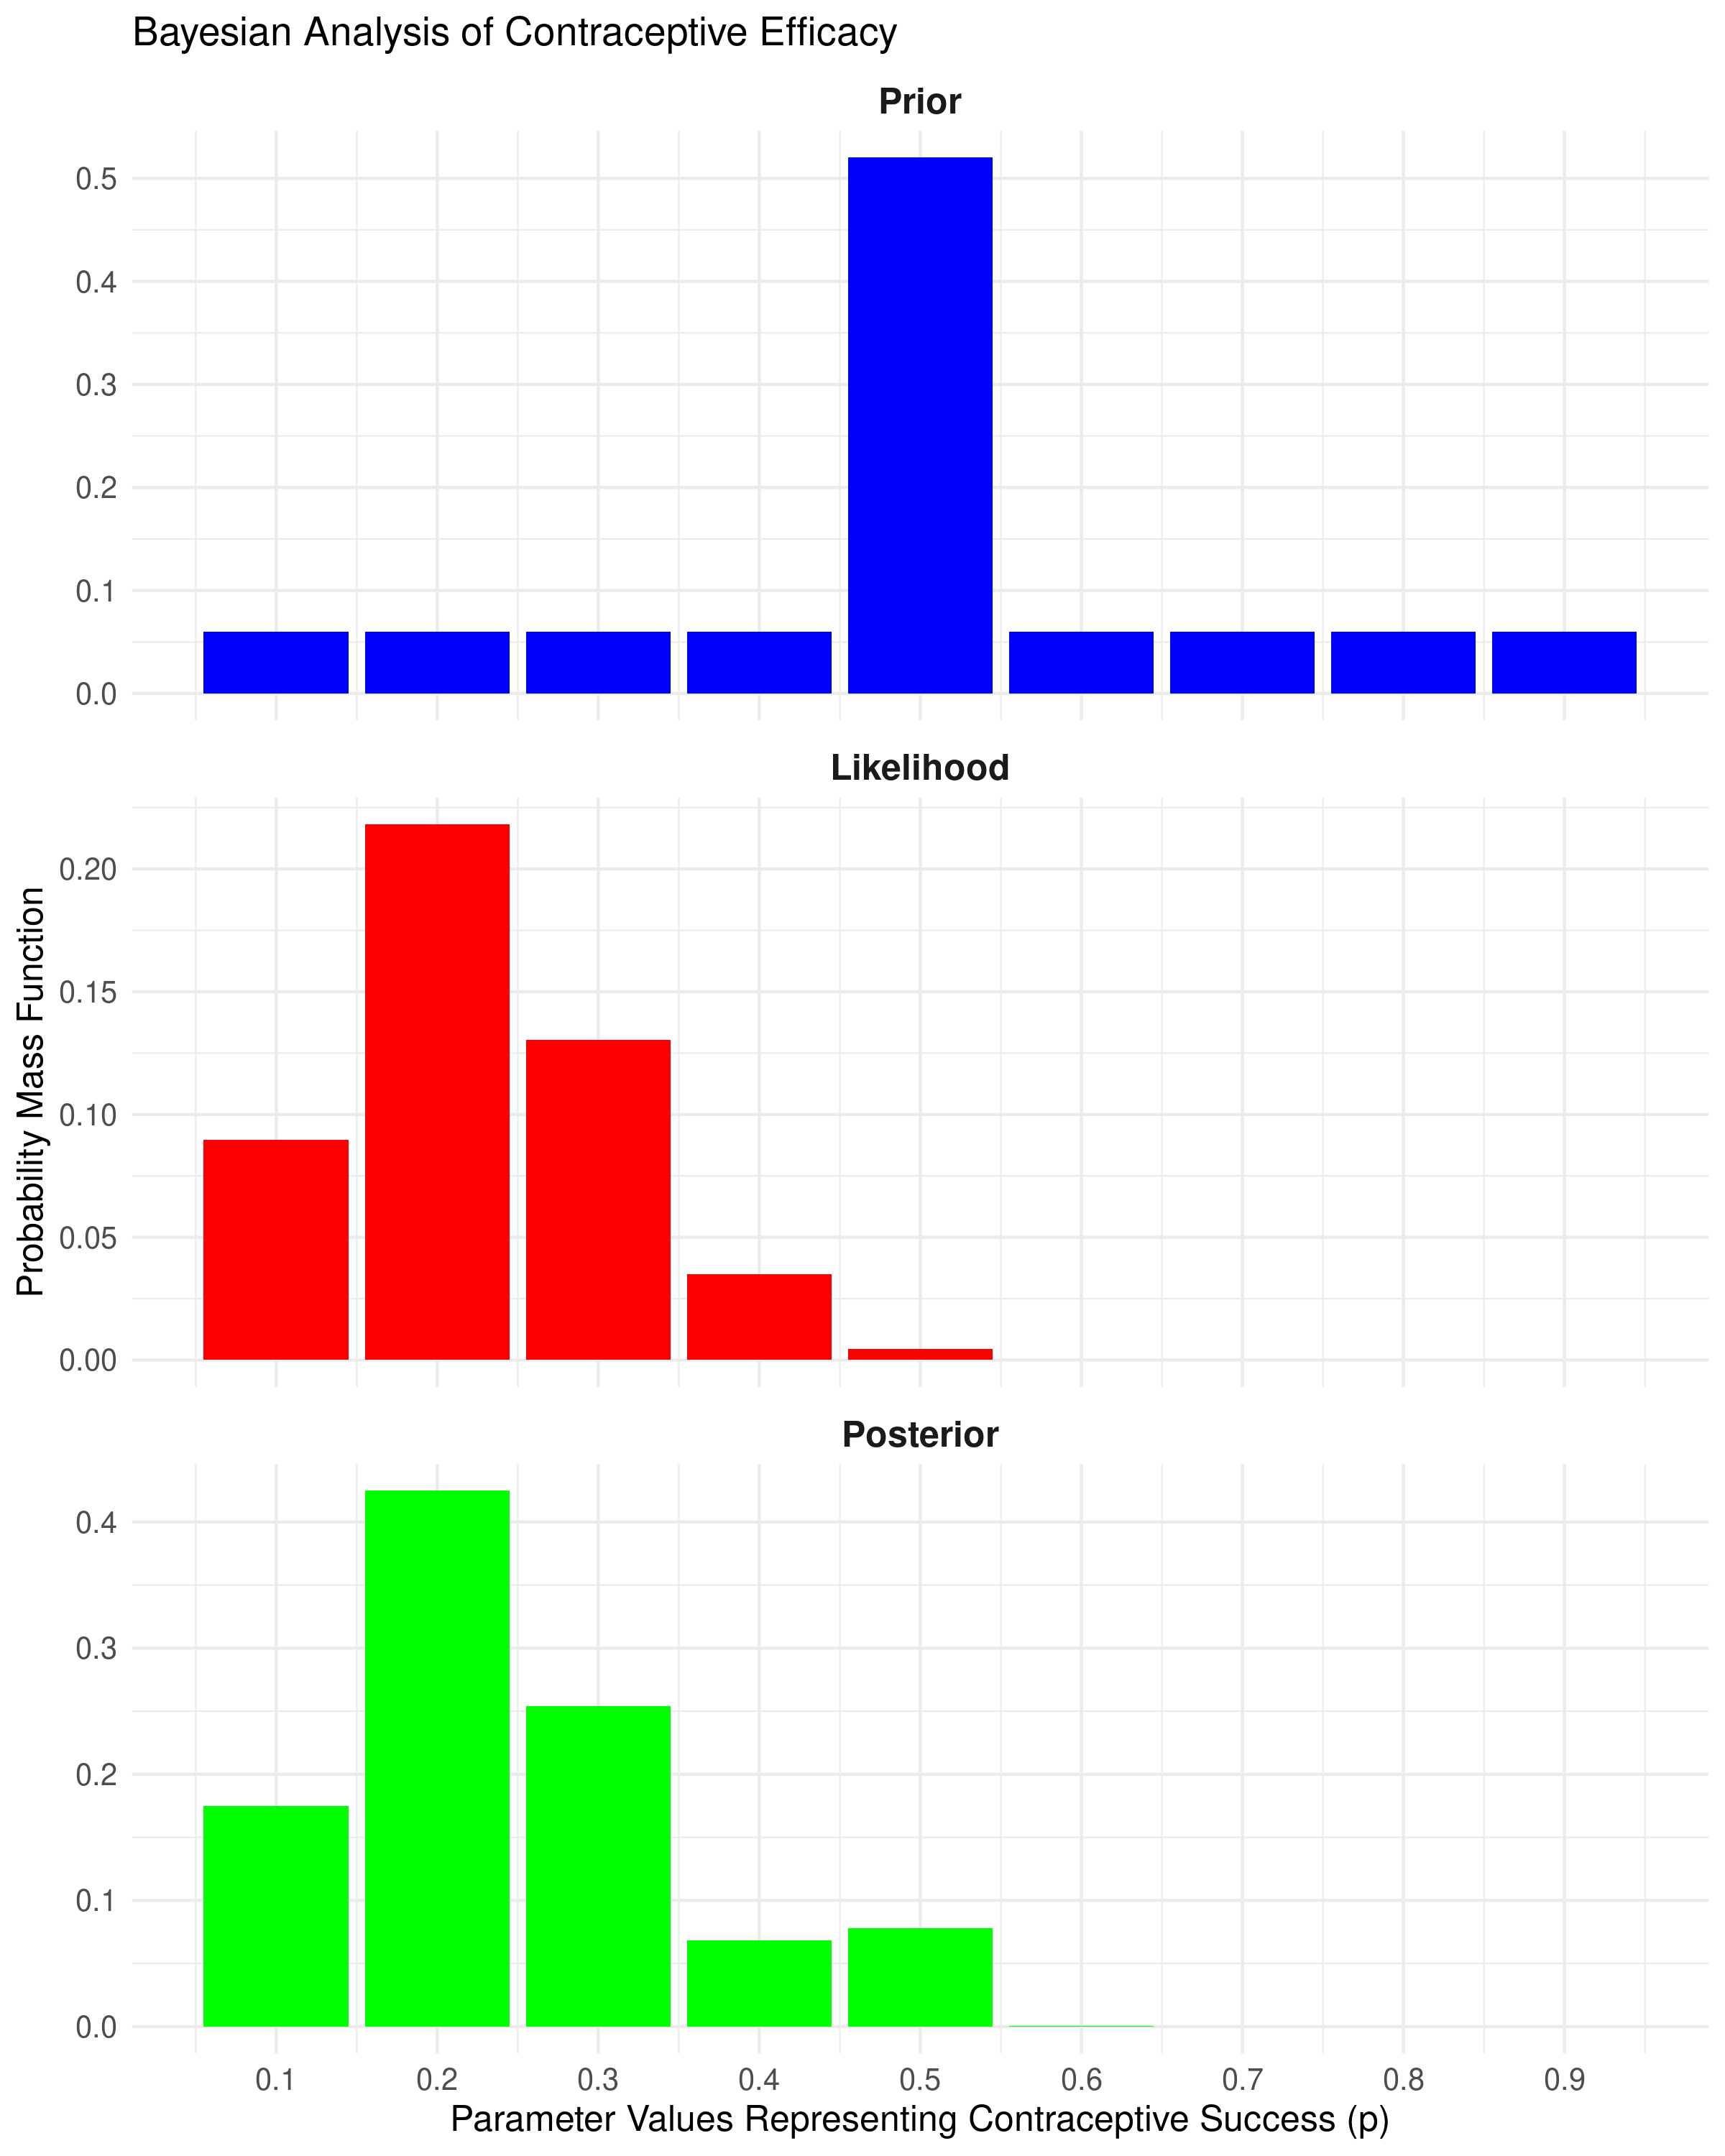
\includegraphics[width=0.8\textwidth]{chapters/chapter1/codes/bayesian_analysis.png} 
    \caption{Code Plots of Prior, Likelihood and Posterior Distributions}
    \label{fig:bayesian_analysis}
\end{figure}

\subsubsection{Effect of Sample Size on the Posterior}

Let's think about what happens to the \textbf{posterior distribution} when we gather more data. Imagine our original scenario: we had 20 samples and observed 4 successes. Now, let's change this slightly and consider a larger sample size of 40 with 8 successes. Importantly, the ratio of successes to the total sample size remains the same at \textit{20\%}.\\

We begin with the same \textbf{prior distribution}. Our goal is to calculate the likelihood of the data, which is still centered at \(0.20\), but because we have more data, the likelihood becomes \textit{less variable}. In other words, there's more certainty about where the true value of \(p\) lies. Once we combine this updated likelihood with the prior, we get the posterior distribution. The result? The posterior is also peaked around \(p = 0.20\), but now the peak is \textbf{taller and narrower}.\\

Why does the peak become taller? This is because with more data, the posterior puts more weight—or probability mass—on values around \(0.20\), and less on values further away. Essentially, we have more confidence that \(p\) is close to \(0.20\).\\

Now, let’s \textit{push this idea further}. Suppose we gather even more data—let's say 200 samples with 40 successes, keeping the same success rate of 20\%. What happens now? The likelihood is again centered at \(0.20\), but it becomes even more concentrated. As a result, almost all of the probability mass in the posterior will now be centered around \(p = 0.20\), with the probability mass for other values of \(p\) shrinking down to nearly zero. The other models don’t have zero probability mass, but their posterior probabilities are extremely close to zero.\\

This illustrates a crucial point: \textbf{as we collect more data, the likelihood becomes more influential than the prior}. In fact, with enough data, the likelihood can \textit{overwhelm} a poor choice of prior. However, there’s an important caveat: this only works if we don’t assign zero probability to any models in the prior. If we completely rule out certain models beforehand, no amount of data will ever shift our belief towards them.\\

So, while a good prior can help, it’s not the end of the world if it's slightly off—more data will gradually correct it. But we must keep an open mind and never assign a zero chance to any possible model in the prior!

\subsection{Example 2: Proportion of M\&M's in Population}

You’ve been hired to make a crucial decision: is the true percentage of yellow M\&M’s in the population \textbf{10\%} or \textbf{20\%}? And here’s the kicker—if you guess right, you get a bonus; if you guess wrong, you're out of a job. No pressure, right? Now, to make this decision, you’re given an option to buy a random sample of M\&M’s, but each sample costs you \$200 per M\&M, and you must buy in \$1,000 increments. That means, every time you sample, you are buying 5 M\&Ms. The total budget? You can spend up to \$4,000, which allows you to buy 5, 10, 15, or 20 M\&M’s.\\

\textbf{What’s the goal?} You want to make a confident decision about the true proportion of yellow M\&M’s, but you also don’t want to spend more money than necessary.\\

\textit{The dilemma:} Data collection is costly, and you don’t want to spend your entire budget if you can make a confident decision with fewer M\&Ms. But at the same time, if you don’t collect enough data, you risk making the wrong decision, which could cost you your job.\\

Let’s break it down mathematically. What you’re essentially trying to do here is a form of hypothesis testing. You’re testing whether the proportion of yellow M\&M’s is \textbf{p = 0.10} or \textbf{p = 0.20}. You want to choose a sample size that gives you a good chance of making the correct decision.\\

If you were to sample just 5 M\&M’s, the observed proportion of yellow M\&M’s might not be enough to give you confidence in your decision. There’s a lot of variability with such a small sample size. But as you sample more, say 10, 15, or 20 M\&M’s, the observed proportion starts to stabilize, giving you more confidence in whether you are dealing with the 10\% or 20\% scenario. Here’s where the idea of a \textit{trade-off} comes into play. More data (i.e., more M\&M’s) reduces the chance of making an error, but it comes at a cost. Fewer data points mean higher uncertainty, but you save money. What you want to do is balance this: sample enough to feel confident, but not so much that you’re wasting resources.\\

One way to approach this is to calculate the probabilities of making the wrong decision for each possible sample size, and then compare that to the cost. Essentially, you’re trying to minimize the \textit{expected loss}—the potential downside of making the wrong decision, combined with the cost of buying more data. \\

The question is: at what point does the reduction in uncertainty outweigh the cost? That’s the sweet spot you want to find. With the right sample size, you’ll be confident in your decision without breaking the bank.

\subsubsection{The Frequentist Approach}

We are going to put the 10\% claim to the test and see if we can gather enough evidence to confidently say whether the true proportion of yellow M\&M’s is more than 10\%.\\

\textbf{Our hypothesis setup:}\\

\(\mathbf{H_0}\) (null hypothesis): The proportion of yellow M\&M’s is 10\%, or \(p = 0.10\).\\
\(\mathbf{H_A}\) (alternative hypothesis): The proportion of yellow M\&M’s is greater than 10\%, or \(p > 0.10\).\\

In statistics, we also need to decide how much uncertainty we are willing to tolerate when making our decision. This is called the \textit{significance level} (\(\alpha\)), and here we are setting it to \(\alpha = 0.05\), which means we’re willing to accept a 5\% chance of making an error in rejecting the null hypothesis.\\

You collect a sample of 5 M\&M’s, and you observe the following colors: red, green, yellow, blue, and orange. Out of these, you see \(\mathbf{k = 1}\) yellow M\&M. So, in a sample of \(\mathbf{n = 5}\), one M\&M is yellow. Now, we compute the \textbf{p-value}, which tells us the probability of observing our data (or something even more extreme) assuming the null hypothesis (\(H_0: p = 0.10\)) is true. In this case, we want the probability of observing at least 1 yellow M\&M out of 5, given that the true proportion is 10\%. This is:

\[
P(k \geq 1 | n = 5, p = 0.10) = 1 - P(k = 0 | n = 5, p = 0.10)
\]

First, calculate the probability of seeing no yellow M\&M’s at all:

\[
P(k = 0 | n = 5, p = 0.10) = (1 - 0.10)^5 = 0.905
\]

So, the p-value is:

\[
P(k \geq 1 | n = 5, p = 0.10) = 1 - 0.90^5 = 0.09^5 \approx 0.41
\]

The p-value of \(\mathbf{0.41}\) means that if the true proportion of yellow M\&M’s is really 10\%, there’s about a 41\% chance we’d see 1 or more yellow M\&M’s in a sample of 5. Since this probability is much higher than our significance level (\(\alpha = 0.05\)), we \textit{fail to reject the null hypothesis}.\\

In other words, the data we collected \textit{do not provide convincing evidence} that the proportion of yellow M\&M’s is greater than 10\%. This doesn’t mean we’ve \textit{proven} that the proportion is exactly 10\%, but it does suggest that, based on our sample, we don’t have enough evidence to confidently claim it’s higher than that.

\subsubsection{The Bayesian Approach}

Here, instead of focusing on a single hypothesis and trying to reject it, we’ll compare two hypotheses directly and update our beliefs based on the data.\\

\textbf{Our hypotheses setup:}\\

\(\mathbf{H_1}\): The proportion of yellow M\&M’s is 10\% (\(p = 0.10\)).\\
\(\mathbf{H_2}\): The proportion of yellow M\&M’s is 20\% (\(p = 0.20\)).\\

In Bayesian inference, we start with \textit{prior probabilities}, which represent our initial beliefs about the hypotheses before we collect any data. Here, we assume no strong preference for either hypothesis, so we assign equal prior probabilities:

\[
P(H_1) = P(H_2) = 0.5
\]

Just like before, we observe 1 yellow M\&M out of 5 M\&M’s (\(\mathbf{k = 1}\) and \(\mathbf{n = 5}\)). Next, we calculate the \textit{likelihoods}, which tell us how probable the observed data is, assuming each hypothesis is true:

\[
P(k = 1 | H_1) = \binom{5}{1} \times 0.10^1 \times 0.90^4 \approx 0.33
\]
\[
P(k = 1 | H_2) = \binom{5}{1} \times 0.20^1 \times 0.80^4 \approx 0.41
\]

With the likelihoods in hand, we can now calculate the \textit{posterior probabilities}, which are our updated beliefs about each hypothesis after observing the data. Using Bayes’ Theorem, the posterior probability of \(\mathbf{H_1}\) is:

\[
P(H_1 | k = 1) = \frac{P(H_1) \times P(k = 1 | H_1)}{P(k = 1)} = \frac{0.5 \times 0.33}{0.5 \times 0.33 + 0.5 \times 0.41} \approx 0.45
\]

Since the probabilities for both hypotheses must sum to 1, the posterior probability of \(\mathbf{H_2}\) is:

\[
P(H_2 | k = 1) = 1 - P(H_1 | k = 1) = 1 - 0.45 = 0.55
\]

After observing 1 yellow M\&M, we find that the posterior probability of \(\mathbf{H_2}\) (20\% yellow M\&M’s) is slightly higher than \(\mathbf{H_1}\) (10\% yellow M\&M’s). In other words, the data nudges us toward believing that 20\% of the M\&M’s are yellow, even though the difference is small. So, if we had to make a decision right now, we’d go with \(\mathbf{H_2}\).\\

Interestingly, this decision is the opposite of what we concluded using the frequentist method. In that case, we failed to reject the null hypothesis of 10\% yellow M\&M’s because the p-value was large. Here, the Bayesian method leans towards 20\%, even though the sample size is small and the difference in posterior probabilities is minor.\\

\textbf{What happens with larger sample sizes?} Let’s see how this plays out if we increase the number of M\&M’s in our sample:

\[
\begin{array}{|c|c|c|c|}
\hline
\textbf{Observed Data (n, k)} & \textbf{Frequentist p-value} & \textbf{Bayesian } P(H_1 | n, k) & \textbf{Bayesian } P(H_2 | n, k) \\
\hline
n = 5, k = 1 & 0.41 & 0.45 & 0.55 \\
n = 10, k = 2 & 0.26 & 0.39 & 0.61 \\
n = 15, k = 3 & 0.18 & 0.34 & 0.66 \\
n = 20, k = 4 & 0.13 & 0.29 & 0.71 \\
\hline
\end{array}
\]

As we collect more data, the frequentist method continues to produce p-values that are larger than our significance level, so we would consistently fail to reject the null hypothesis of 10\%. Meanwhile, the Bayesian approach steadily increases the posterior probability for \(\mathbf{H_2}\) (20\% yellow M\&M’s) as we gather more evidence.\\

\textbf{A key insight:} This example highlights a subtle but important difference between the two approaches. The \textit{frequentist method} is highly sensitive to how we define our null and alternative hypotheses. If we had flipped them—testing whether the proportion is less than 20\%—we might have arrived at a different decision. On the other hand, the \textit{Bayesian method} updates our beliefs consistently, no matter how we set up the problem. This flexibility makes Bayesian inference particularly powerful when dealing with uncertain data and competing hypotheses.



